\section{Resultados obtenidos}

A continuación, se presentan los resultados de cada submódulo luego de ser sometido en las pruebas creadas para cada uno, mencionadas en la sección del plan de pruebas.
Se van a mostrar las pruebas más significativas, de tal forma que evidencien el funcionamiento esperado de cada submódulo.
Al final se muestran los resultados para el PCS completo.

\subsection{Módulo \texttt{TRANSMIT}}

Para la verificación del funcionamiento del módulo transmisor, se muestra la prueba 0: \textit{IDLEs después de reset} y la prueba 1: \textit{Carrier extend y IDLE con disparidad correcta}, así como la prueba 2: \textit{Sin carrier extend e IDLE con disparidad errónea} y prueba 3: \textit{Sin carrier extend e IDLE con disparidad correcta}.

En la Figura \ref{fig:transmit_prueba0y1}, se muestra como primera prueba el envío de IDLEs.
Después de un reinicio, como se indica en el estándar IEEE 802.3, el transmisor comienza con disparidad negativa y se envían IDLEs (\texttt{/I/}).
Cuando se activa \texttt{tx\_en}, se envía la condición de inicio \texttt{/S/} y comienza el envío de la trama de datos.

En la prueba 1, por los \textit{code-groups} enviados, se requiere realizar un ajuste de paridad de ciclos (\textit{carrier extend}) y se envía un \texttt{/R/} extra para que el IDLE siguiente comience en ciclo par.

En la prueba 2, al finalizar con disparidad incorrecta, se envía el /D5.6/ y se corrige la disparidad, que es el comportamiento esperado.
Finalmente en la prueba 3, no hay \textit{carrier extend} ni disparidad incorrecta (está el /D16.2/).
Por lo tanto, esta muestra de las pruebas cumple con el plan establecido.

\begin{figure}[H]
    \centering
    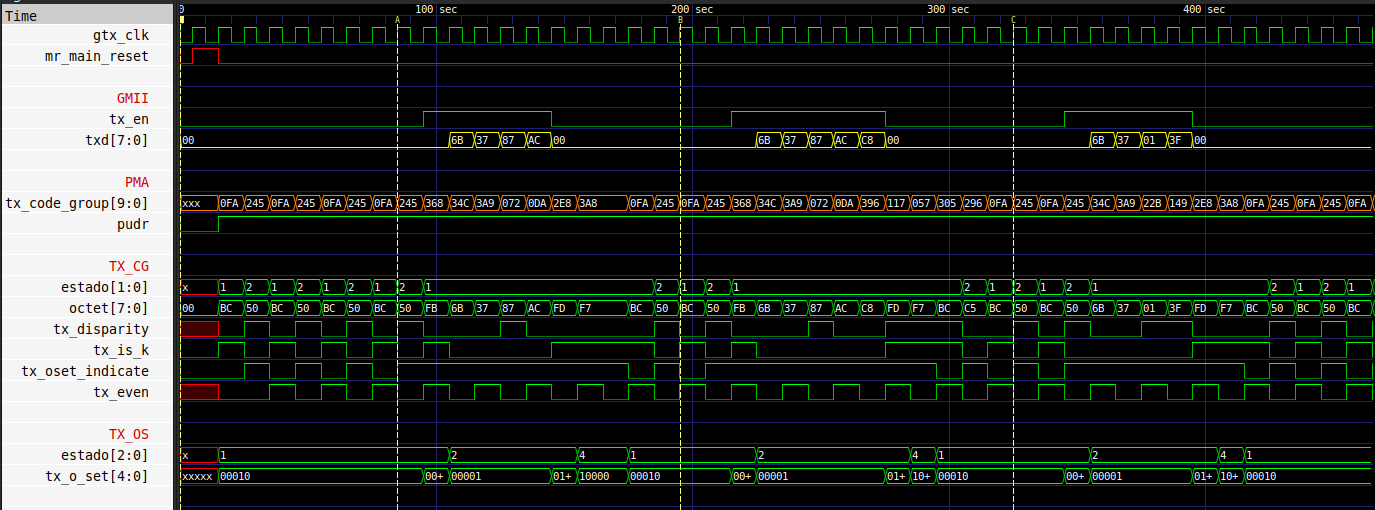
\includegraphics[width=\textwidth]{images/pruebas_transmit.png}
    \caption{Ejecución de prueba 0, 1, 2 y 3 para el \texttt{TRANSMIT}.}
    \label{fig:transmit_prueba0y1}
\end{figure}

\subsection{Módulo \texttt{SYNCHRONIZATION}}


Primero, se muestran los resultados para las pruebas 1 y 2.
Se verifica el correcto funcionamiento del módulo a la hora de recibir las \texttt{COMMA} para la sincronización inicial, entrando al estado de \texttt{SYNC\_ACQUIRED\_1}. Las pruebas se pueden observar en la primera parte de la Figura \ref{pruebaSYNC}.
\begin{figure} [H]
    \centering
    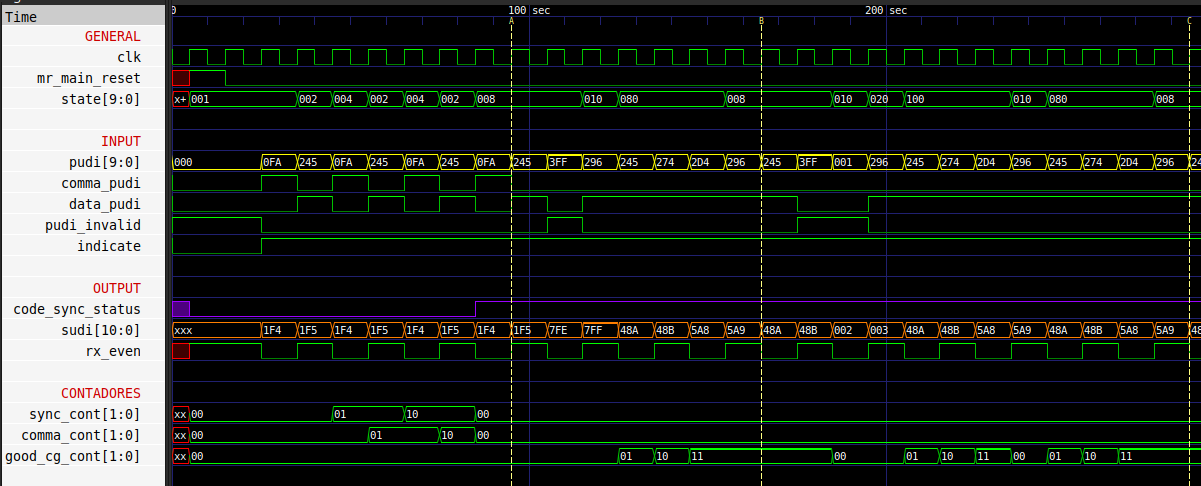
\includegraphics[width=1\linewidth]{images/prueba1_2_y_3_sync.png}
    \caption{Prueba de sincronizaci\'on completa al recibir 3 \textit{comas}}
    \label{pruebaSYNC}
\end{figure}

En la segunda parte de la figura anterior, se ingresa un dato inválido y se vuelve a sincronizar con 4 datos válidos, lo cual cumple exactamente con el comportamiento esperado.
Observe que no se pierde la sincronización completamente (\texttt{code\_sync\_status} = 0), el cual es el comportamiento esperado.

En la Figura \ref{pruebaSYNC2}, se muestran los resultados de las pruebas 5 y 6.
En la prueba 5, se envía un dato inválido y después al intentar volver al estado estable de sincronización, se envía otro.
Por lo tanto, se requiere recibir 8 datos válidos para volver a sincronizarse completamente.
Después de volver al estado \texttt{SYNC\_ACQUIRED\_1}, se realiza la prueba 6, que corresponde a la pérdida de sincronización completa.
Para ello, se envían 4 code-groups inválidos y se transiciona al estado \texttt{LOSS\_OF\_SYNC}.
Para el sincronizador, también se concluye que las pruebas realizadas fueron exitosas y se determinó su funcionamiento correcto según el estándar.

\begin{figure} [H]
    \centering
    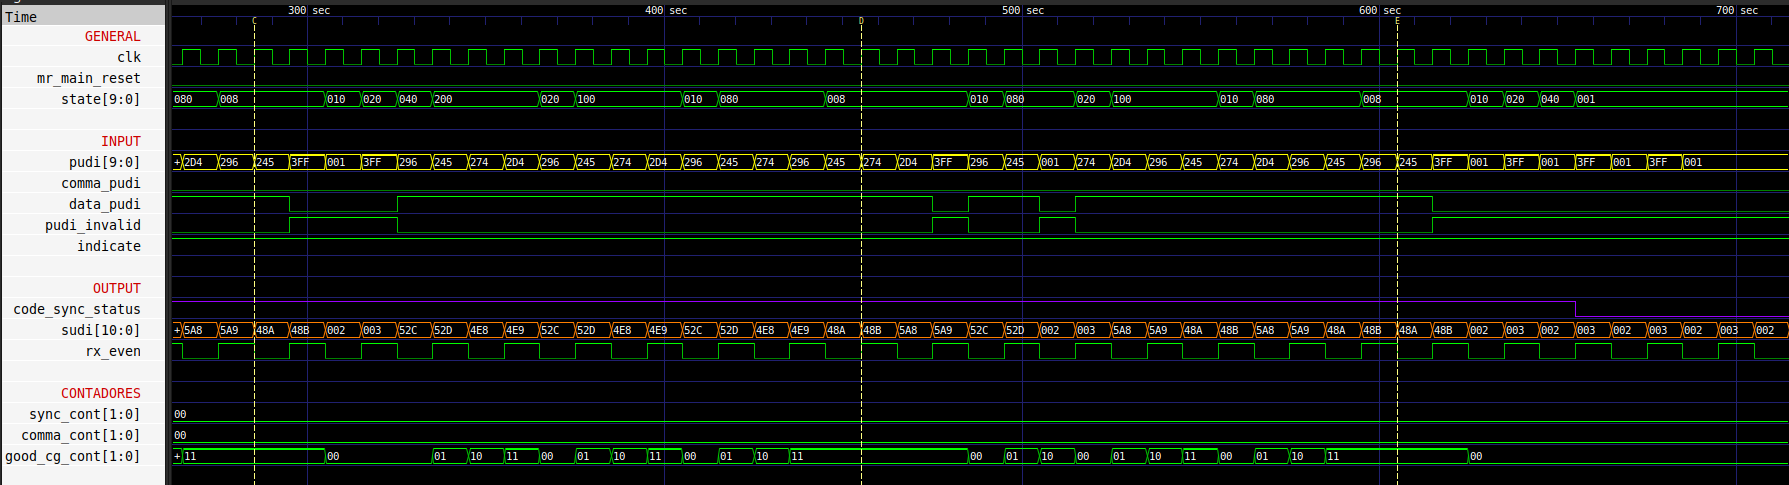
\includegraphics[width=1\linewidth]{images/prueba4_5_y_6_sync.png}
    \caption{Prueba al recibir datos err\'oneos}
    \label{pruebaSYNC2}
\end{figure}


\subsection{Módulo \texttt{RECEIVE}}

Los resultados del módulo \texttt{RECEIVE} se muestran a continuación.

\subsubsection{Envío de datos}
\begin{figure}[H]
    \centering
    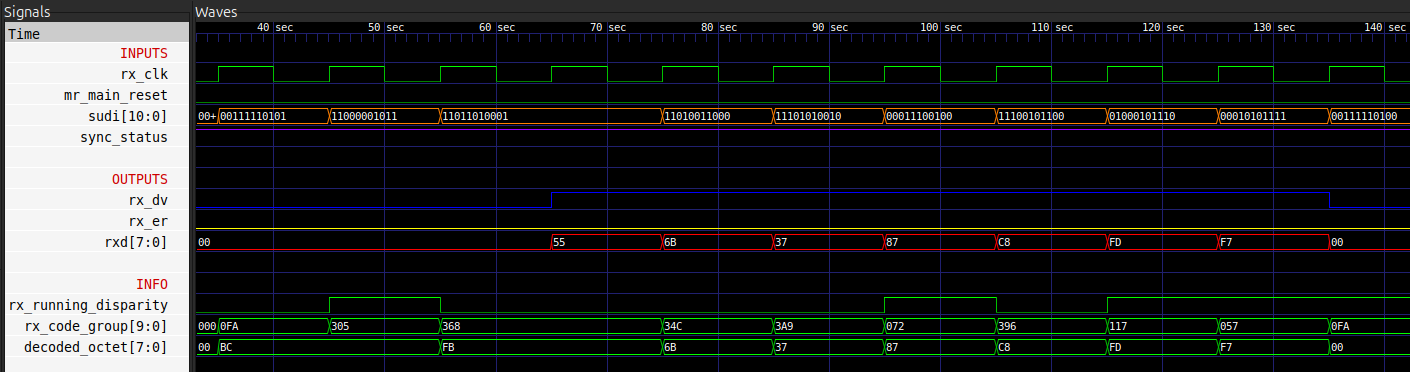
\includegraphics[width=0.9\linewidth]{images/prueba1_receive.png}
    \caption{Resultados obtenidos en la prueba de envío de datos.}
    \label{fig_prueba1_receive}
\end{figure}
\indent En la Figura \ref{fig_prueba1_receive} se puede observar los resultados obtenidos luego del envío de datos, en la señal de color naranja se puede observar la entrada SUDI, la cual trae consigo el rx code group, se puede observar que cuando se recibe la señal de start se activa la salida \texttt{rx\_dv}, la cual es la señal de color azul, y se envía a través de la señal rxd, la cual está de color rojo, un valor de 55, el cual viene mencionado en el estándar que se debe de enviar en el estado de start, seguido a esto se reciben los datos que se mencionaron en el Cuadro \ref{prueba1_receive} y se puede observar que rxd está enviando de manera correcta el octeto específico. Así también cuando se envía un T/R/I deja de enviar datos, ya que esto significa que ya se ha concluido el envío de datos.

\subsubsection{Envío de datos, pero el receptor no está sincronizado}
\indent Al realizar esta prueba se obtuvieron los resultados esperados, por lo que se concluye que el receptor no fallaría si se le presenta esta situación.

\subsubsection{Terminación /T/R/R/}
\indent Al realizar esta prueba los resultados fueron los esperados, ya que efectivamente el receptor detectó la secuencia /T/R/R y en el siguiente ciclo de reloj se activó la señal rx er y rxd tomó el valor de 0x0F y seguidamente terminó el envío de datos.

\subsection{PCS completa}

En cuanto a los resultados aplicados a la PCS completa, se determinaron satisfactorios y se obtuvo el resultado esperado.
Las pruebas realizadas son similares a las aplicadas en el módulo de \texttt{TRANSMIT} individualmente.

En la Figura \ref{fig_prueba_1_pcs}, se muestra inicialmente la sincronización en el primer bloque, donde se reciben caracteres /K28.5/ y finalmente se activa \texttt{code\_sync\_status}.
Luego, se realiza el envío de una trama que tiene que aplicar \textit{carrier extend}. Se observa que efectivamente tiene un envío correcto de esta y la decodificación es exitosa en \texttt{rxd}.
En la tercera prueba de la figura, se envía una trama que no requiere \textit{carrier extend}.
Por lo tanto, estos resultados fueron los esperados para la prueba 0, 1 y 2.

\begin{figure}[H]
    \centering
    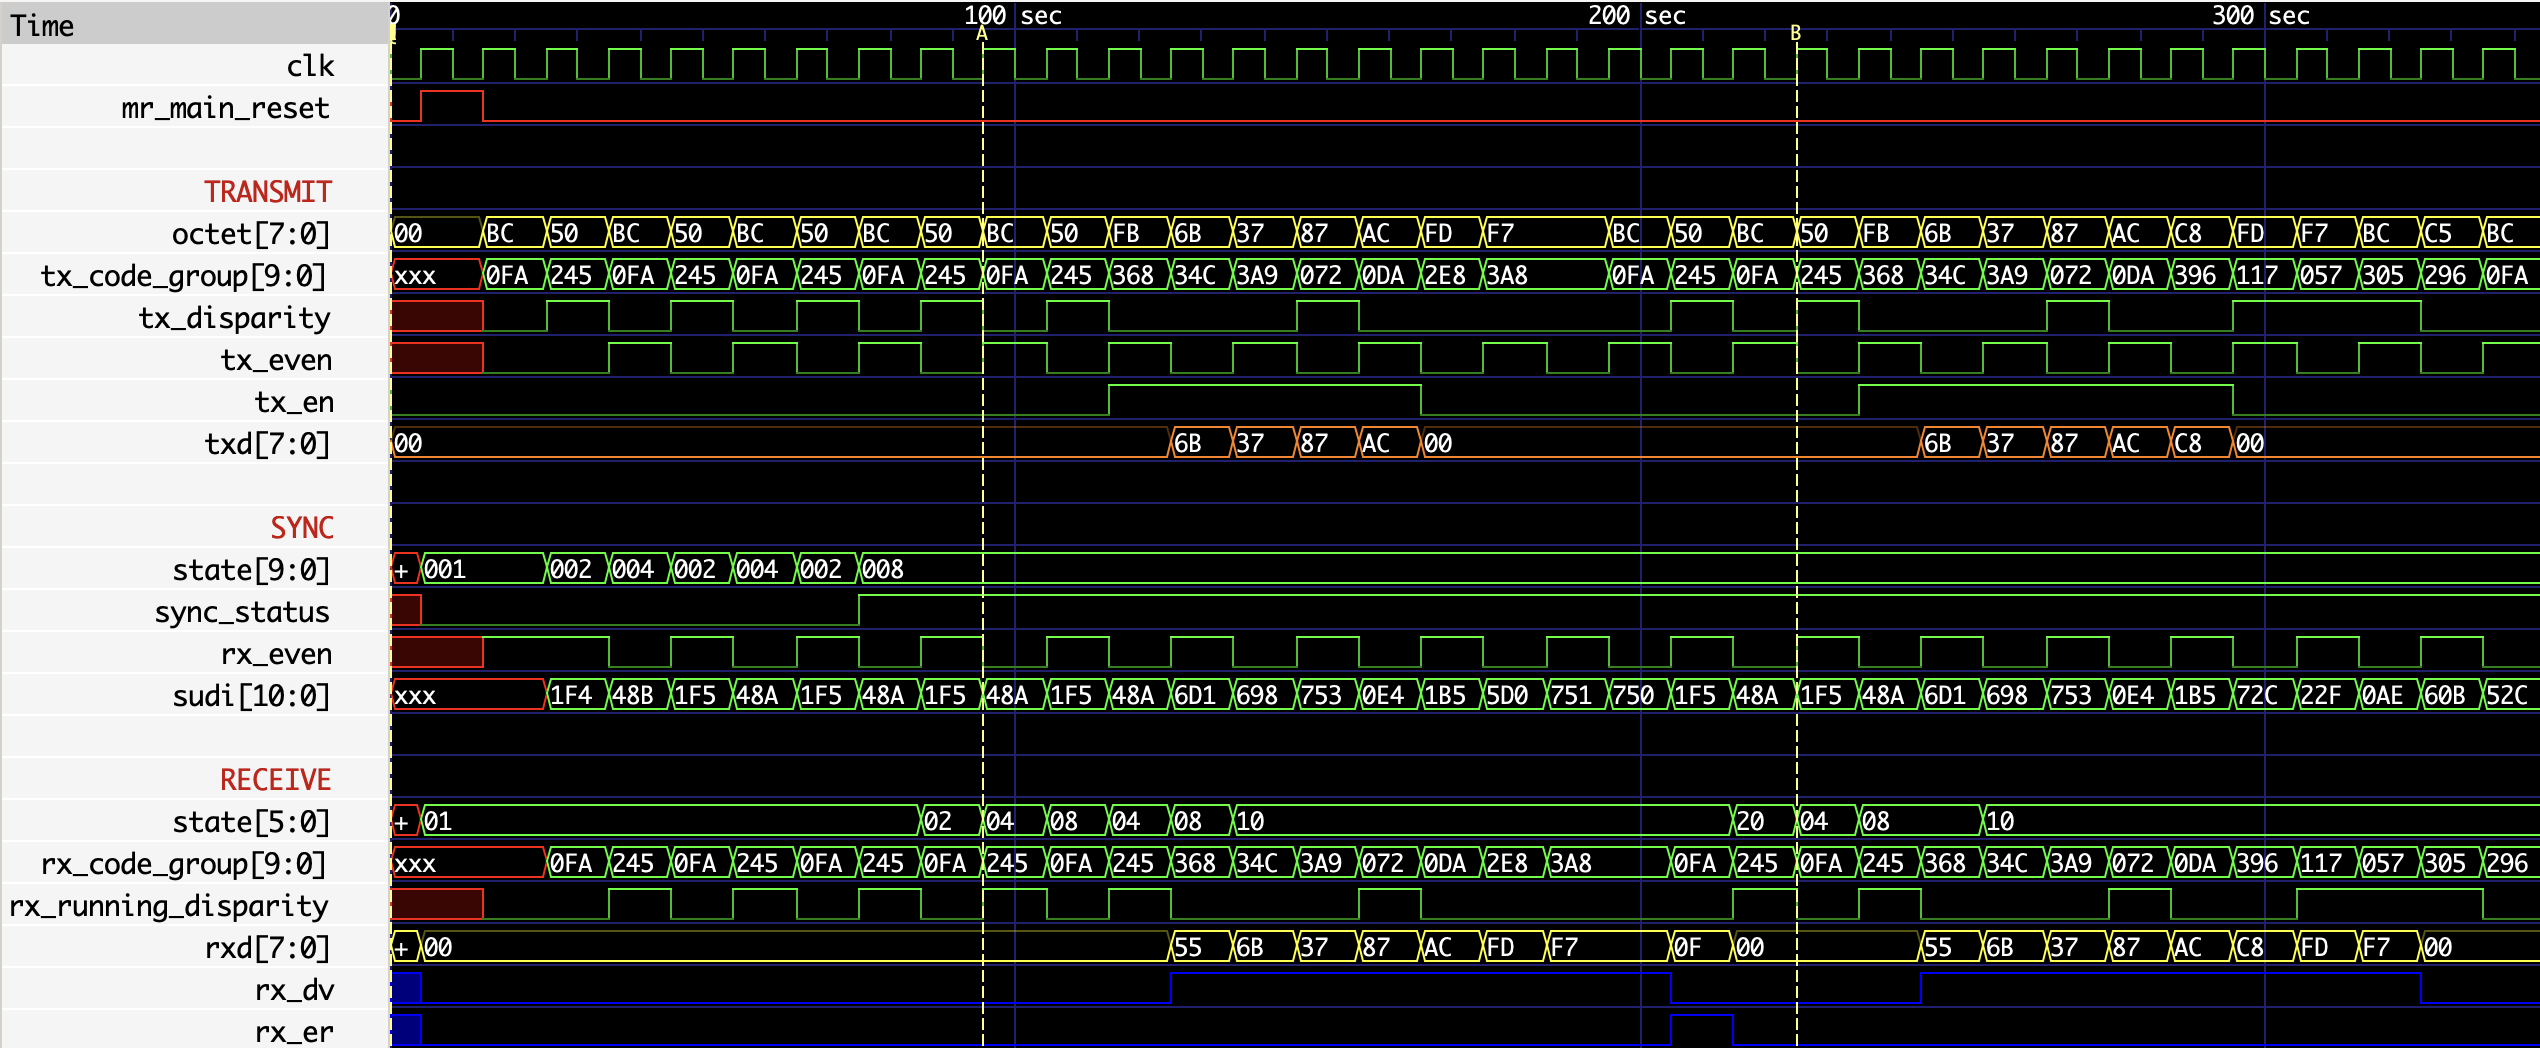
\includegraphics[width=\linewidth]{images/pruebas_pcs_1.png}
    \caption{Prueba de sincronización, envío de trama con \textit{carrier extend} y sin \textit{carrier extend}.}
    \label{fig_prueba_1_pcs}
\end{figure}

Luego, en la Figura \ref{fig_prueba_2_pcs}, se realiza el envío de todos los code-groups que fueron seleccionados (prueba 4), para verificar su correcta codificación y decodificación.
En la prueba 5, mostrada al final de la imagen, se envían los code-groups inválidos descritos en la sección del plan de pruebas y se observa que se pierde la sincronía después de 4 inválidos.
Acá, \texttt{rxd} está en bajo y \texttt{rx\_dv} está en bajo.

\begin{figure}[H]
    \centering
    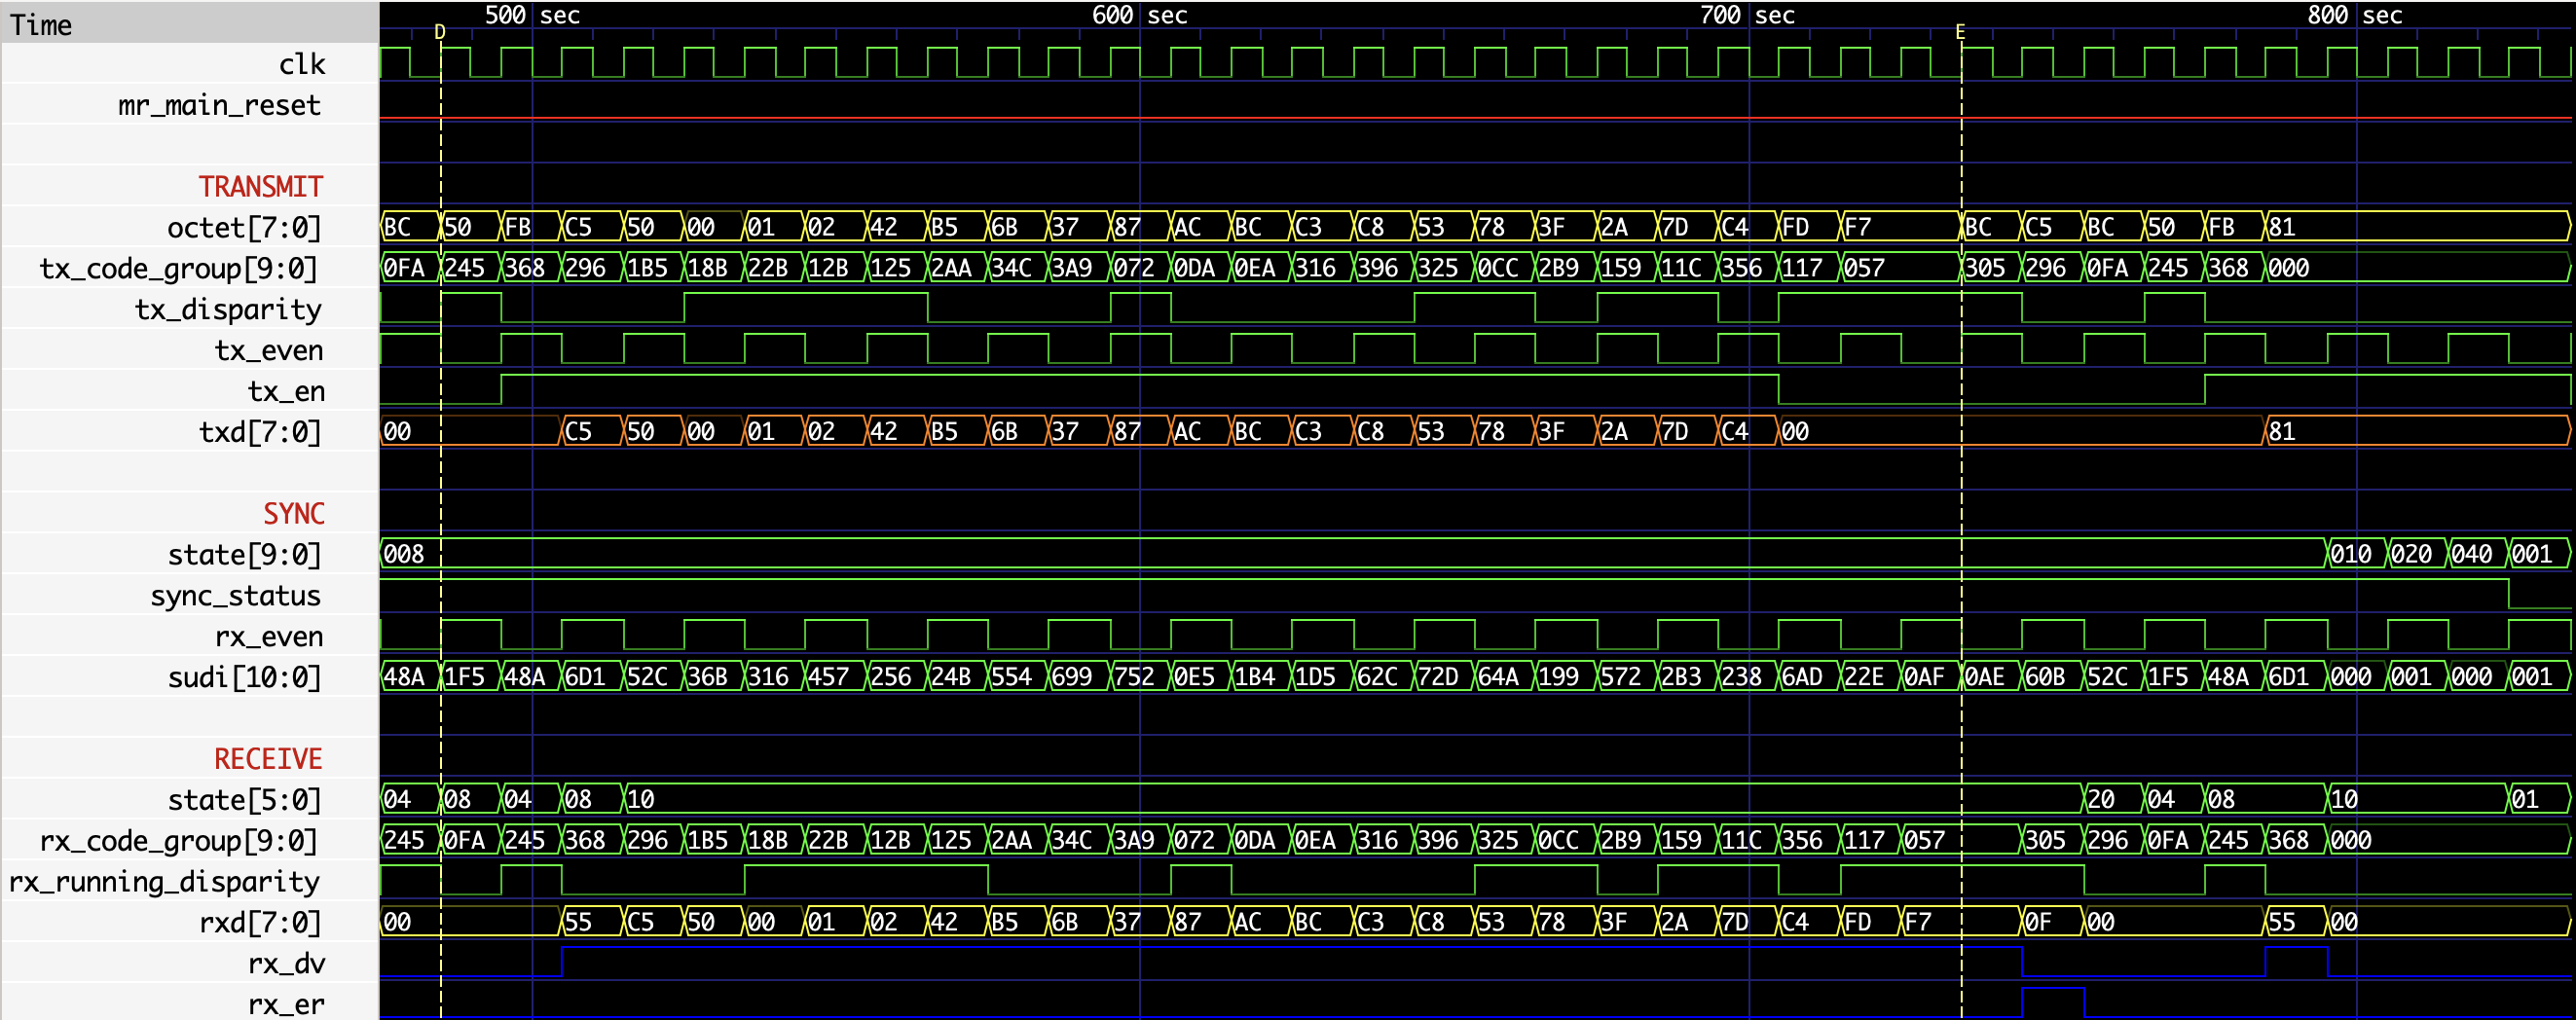
\includegraphics[width=\linewidth]{images/pruebas_pcs_2.png}
    \caption{Prueba de envío de todos los code-groups seleccionados y pérdida de sincronía.}
    \label{fig_prueba_2_pcs}
\end{figure}